Constructing intelligent programs that play games with imperfect information is challenging --- two notorious examples that have recently stirred some interest being Hanabi~\cite{DBLP:journals/corr/abs-1902-00506} and Starcraft~2~\cite{DBLP:conf/ijcai/HuLLPX18}. As far as we know, an important ingredient that misses from most approaches is the ability to reason about higher-order knowledge (an agent knows that another agent knows that\dots). In these systems, epistemic logic and its dynamic extension, \emph{dynamic epistemic logic} (DEL) \cite{baltag1998logic}, \cite{DitmarschvdHoekKooi} may offer formal tools for providing explanations in such AI programs. 
% ALEX j'ai vire la phrase qui est incomplete
%needs to be understood is relevant in AI, especially in strategic reasoning \cite{DBLP:journals/ijgt/Aumann99}.

The only pedagogical tool explaining these models that we are aware of is \emph{Hintikka's world}, which was presented at ECAI-IJCAI~2018~\cite{DBLP:conf/ijcai/Schwarzentruber18}. 
\emph{Hintikka's world} is a proof of concept of a graphical user interface that represents Kripke models by  comic strips, as shown in Figure \ref{figure:gui}. It enables the user to explore the mental states of agents. The tool is available at the following address:
\url{http://hintikkasworld.irisa.fr/} and the source code is available here:
\url{https://gitlab.inria.fr/fschwarz/hintikkasworld}


Kripke models are graphs, represented explicitly in memory in the first version of the tool. Explicit models are useful to learn how dynamic epistemic logic works, by means of toy examples: ``Muddy Children'', ``Sally and Anne''~\cite{wimmer1983beliefs}, etc.  However, the first version of Hintikka's world does not \emph{scale}. For instance, in real card games, such as Hanabi, there is an exponential number of possible configurations of cards. In its standard version, Hanabi has 50 cards total, each player's hand contains 4 cards, and the order of the cards is important. Therefore, with 4 players, the initial Kripke model features $50 \times 49 \times 48 \times \dots \times 35$ configurations, that is %$2.2 \times 10^{21}$.
$1.03 \times 10^{26}$.
Thus, it is impossible to explicitly represent the full graph in memory.



That is why, in this demonstration, we propose to represent Kripke models \emph{symbolically} by using the approach of \citeauthor{DBLP:conf/atal/CharrierS17}~\shortcite{DBLP:conf/atal/CharrierS17,DBLP:conf/aiml/CharrierS18}. The implementation relies on Binary Decision Diagrams (BDDs) \cite{DBLP:journals/tc/Bryant86}. There is another implementation of symbolic epistemic models, called DEMO \cite{DBLP:conf/lori/BenthemEGS15}, but their implementation is difficult to use in a web application and has no graphical user interface. %\cite{papadimitriou2003computational}






\begin{figure}
	\begin{center}
		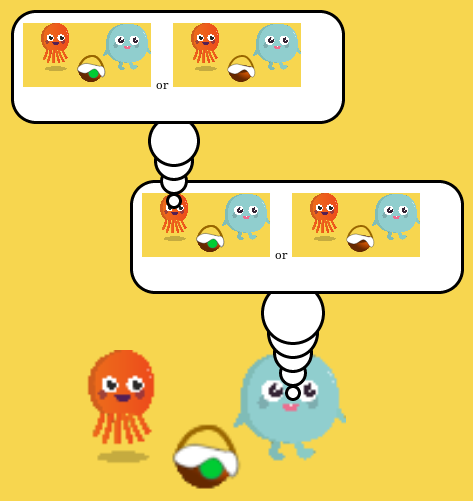
\includegraphics[width=1.8cm]{images/screenshot.png}
		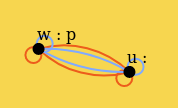
\includegraphics[width=3cm]{images/hintikkas_world_epistemicmodel.png} 
	\end{center}
	\caption{Graphical user interface of \emph{Hintikka's world}.\label{figure:gui}}
\end{figure}
